\input qpd-bootstrap

\begin{problem}{20260811}
  \meta{name}{Vector Triangles and Their Simple Applications}
  \meta{setter}{Ryan Huang, Sophie Chen}
  \meta{score}{7}
  \meta{topic}{Mechanics}
  \meta{difficulty}{3}
  \meta{tags}{mechanics, kinematics, projectile motion}

    
\emph{The vector triangle is a practical and common tool in physics, yet it barely appears in AP examinations.  What follows is a brief introduction, a worked example, and a set of problems for the reader to explore.}

\subsection*{Concept and Example}

Consider the following scenario.  A point mass $m$ is launched from the ground at an angle $\theta$; its initial velocity $\arr{v}_{0}$ is the leftmost vector in Figure~1.  Throughout the motion a constant downward acceleration of magnitude $g$ acts on the body --- that is the vector on the right of the $+$ sign in the figure.  At landing the velocity is the vector to the right of the $=$ sign.  The whole evolution can therefore be synthesised into the triangle shown on the right.

\begin{center}
    \begin{minipage}{0.85\textwidth}
    \centering
    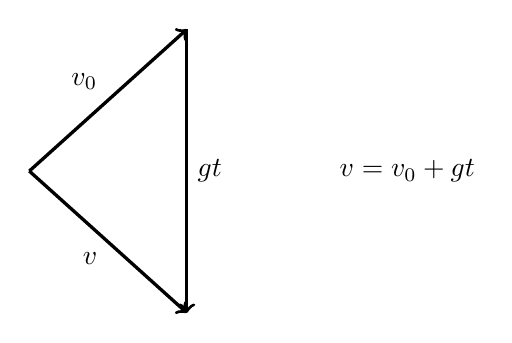
\begin{tikzpicture}[scale=1]
      % -- v0 (launch) --
      \draw[->,very thick] (0,0) -- (2,1.8)
        node[midway,above left] {$\arr{v}_{0}$};
      % -- gt (straight down from tip of v0) --
      \draw[->,very thick] (2,1.8) -- (2,-1.8)
        node[midway,right] {$\arr{g}t$};
      % -- v (final, tip-to-tail from origin) --
      \draw[->,very thick] (0,0) -- (2,-1.8)
        node[midway,below left] {$\arr{v}$};
      % -- label --
    
      \node at (4.8,0) {$\arr{v} = \arr{v}_{0} + \arr{g}t$};
    \end{tikzpicture}
    \par\smallskip
    \textit{Fig.~1 --- The vector triangle for ground-to-ground projectile motion.  $\arr{v}_{0}$ and $\arr{g}t$ have fixed directions; $\arr{v}$ and the flight time $t$ vary with $\theta$.}
    \end{minipage}
\end{center}

This construction leads to a classic question: at what angle $\theta$ must one launch the mass to maximise the horizontal range?  Intuition (and elementary kinematics plus trigonometry) gives $45^{\circ}$.  Here we offer a different approach --- using the \emph{area} of the vector triangle.

Integrating velocity gives displacement, so let us examine the area of the triangle formed by $\arr{v}_{0}$, $\arr{g}t$, and $\arr{v}$.  A short calculation (left to the reader in Q1 below) shows that
\[
  S = \tfrac{1}{2}\,gx, \tag{3}
\]
where $x$ is the horizontal range.  Notice that the area depends \emph{only} on $x$; once we express $S$ in terms of the launch parameters, maximising $x$ reduces to maximising the area of a triangle with two sides of fixed length.

Indeed, in our triangle one side ($\arr{g}t$) changes with the flight time, but another view fixes $\arr{v}_{0}$ and varies the angle $\alpha$ between $\arr{v}_{0}$ and $\arr{v}$.  A second calculation (Q2) yields
\[
  S = \tfrac{1}{2}\,v_{0}^{2}\sin 2\theta
    = -\tfrac{1}{2}\,v_{0}^{2}\sin 2\alpha. \tag{4}
\]
From either expression the maximum occurs at $\theta = 45^{\circ}$, recovering the familiar result through a purely geometric route.

\newpage

\subsection*{Problems}

The following exercises walk you through the derivation sketched above and extend the idea to a slightly more general setting.

\begin{assumptions}
  \item Flat, level ground; uniform gravity $\arr{g} = -g\,\hat{\mathbf{y}}$; no air resistance.
  \item The vector triangle is formed by $\arr{v}_{0}$, $\arr{g}t$, and $\arr{v}$ at the instant of landing ($y = 0$).
  \item In Q3 the launch point is elevated: $y(0) = h$, $y(t_{\text{land}}) = 0$.
\end{assumptions}

\begin{questions}
  \item \textbf{Area in terms of range.}
        Consider the same scenario as the example above (ground-to-ground).
        Prove that the area of the vector triangle is
        \[
          S = \tfrac{1}{2}\,gx,
        \]
        where $x$ is the horizontal range of the projectile.

  \item \textbf{Area in angular form.}
        For the same scenario, show that the area can also be written as
        \[
          S = \tfrac{1}{2}\,v_{0}^{2}\sin 2\theta
            = -\tfrac{1}{2}\,v_{0}^{2}\sin 2\alpha,
        \]
        where $\alpha$ is the angle between $\arr{v}_{0}$ and $\arr{v}$.  Use either expression to confirm that the range is maximised at $\theta = 45^{\circ}$.

  \item \textbf{Non-zero launch height.}
        Now the mass is launched from $y = h > 0$ and lands at $y = 0$ (all else unchanged).  Determine the angle $\theta$ that maximises the horizontal distance $L$.  No resistance of any kind.

        \textit{Hint:} the vector-triangle idea generalizes --- think about what changes when the launch and landing heights differ.
\end{questions}

\end{problem}

\begin{solution}{20260811}

\subsection*{Q1. Area in terms of range}

Let the flight time be $t$.  Resolving the initial velocity,
\[
\arr{v}_{0} = (v_{0}\cos\theta, v_{0}\sin\theta),
\qquad
\arr{g}t = (0, -gt).
\]

The cross-product magnitude of any two sides of the triangle gives (twice) its area.  Choosing $\arr{v}_{0}$ and $\arr{g}t$,
\[
2S = \abs{\arr{v}_{0} \times (\arr{g}t)}
    = \abs{(v_{0}\cos\theta)(-gt) - (v_{0}\sin\theta)(0)}
    = gtv_{0}\cos\theta.
\]

Since $x = v_{0}\cos\theta \cdot t$ is precisely the horizontal range, hence
\[
\boxed{S = \tfrac{1}{2}gx}.
\]

\subsection*{Q2. Area in angular form}

For ground-to-ground motion, the vertical displacement is zero:

\[
0 = v_{0}\sin\theta \cdot t - \tfrac 1 2 gt^{2}
\;\Longrightarrow\;
t = \frac{2v_{0}\sin\theta}{g}.
\]

Substituting into the area formula of Q1,
\[
S = \tfrac{1}{2}\,g\,(v_{0}\cos\theta)\,
      \frac{2v_{0}\sin\theta}{g}
  = \boxed{\tfrac{1}{2}\,v_{0}^{2}\sin 2\theta}.
\]

Now consider the same triangle but with the two sides $\arr{v}_{0}$ and
$\arr{v}$ meeting at the origin.  For ground-to-ground motion, energy
conservation gives $\abs{\arr{v}} = \abs{\arr{v}_{0}} = v_{0}$.  The
(signed) area of the triangle is
\[
S = \tfrac{1}{2}\,\abs{\arr{v}_{0}}\,\abs{\arr{v}}\,\sin\alpha
  = \tfrac{1}{2}\,v_{0}^{2}\sin\alpha,
\]
where $\alpha$ is the interior angle at the origin, taken from $\arr{v}_{0}$
to $\arr{v}$.  At landing $\arr{v} = (v_{0}\cos\theta,\,-v_{0}\sin\theta)$,
so $\alpha = -2\theta$ (the velocity has rotated clockwise by $2\theta$).
Hence
\[
\sin\alpha = \sin(-2\theta) = -\sin 2\theta,
\qquad
S = -\tfrac{1}{2}\,v_{0}^{2}\sin\alpha.
\]

The two forms are therefore equivalent:  $\boxed{S
= \tfrac{1}{2}v_{0}^{2}\sin 2\theta
= -\tfrac{1}{2}v_{0}^{2}\sin\alpha}$.

The maximum of $S$ --- and therefore of $x$ --- occurs when $\sin 2\theta = 1$,
i.e.\ $\boxed{\theta = 45^{\circ}}$, recovering the familiar result through a
purely geometric route.

\subsection*{Q3.  Non-zero launch height}

The mass is launched from $y = h > 0$ and lands at $y = 0$.  The flight time
satisfies
\[
0 = h + v_{0}\sin\theta \cdot t - \tfrac{1}{2}gt^{2},
\]
giving
\[
t(\theta) = \frac{v_{0}\sin\theta
                + \sqrt{v_{0}^{2}\sin^{2}\theta + 2gh}}{g}.
\]

The horizontal range is $L(\theta) = v_{0}\cos\theta \cdot t(\theta)$.

To maximise $L$, set $\dd L/\dd\theta = 0$.  Writing $L$ explicitly and
differentiating (or, more elegantly, using the implicit relation
$L\tan\theta - gL^{2}/(2v_{0}^{2}\cos^{2}\theta) + h = 0$ obtained by
eliminating $t$), one finds
\[
\boxed{\sin^{2}\theta_{\text{opt}}
       = \frac{v_{0}^{2}}{2(v_{0}^{2} + gh)}}.
\]

Equivalently,
\[
\theta_{\text{opt}} = \arcsin\sqrt{\frac{v_{0}^{2}}{2(v_{0}^{2}+gh)}},
\qquad\text{or}\qquad
\tan\theta_{\text{opt}} = \frac{v_{0}}{\sqrt{v_{0}^{2} + 2gh}}.
\]

\medskip
\noindent\textit{Geometric note.}
From Q1, $S = \tfrac{1}{2}gL$ still holds.  Energy conservation gives
$\abs{\arr{v}}^{2} = v_{0}^{2} + 2gh$, so the two sides meeting at the origin
have \emph{fixed} lengths $v_{0}$ and $\sqrt{v_{0}^{2}+2gh}$.
The area $S = \tfrac{1}{2}v_{0}\abs{\arr{v}}\sin\varphi$ (where $\varphi$
is the angle between $\arr{v}_{0}$ and $\arr{v}$) is maximised when
$\varphi = 90^{\circ}$, i.e.\ when $\arr{v}_{0} \perp \arr{v}$.
Imposing orthogonality on the vector triangle yields the same optimal angle
as above, without calculus.

\end{solution}

\input qpd-end
